% !TEX root = ../paper.tex
\section{Interaction techniques} \label{sec:techniques}
In this section we illustrate and describe techniques that can be used to push information from handheld devices to large displays with the purpose of empirically comparing them to each other.
We want to find intuitive techniques that allow a user to walk up and use a large display.
The techniques are characterized by allowing the users to interact with a large screen in a natural way using one or both hands and their mobile phone.

All the techniques were found in the literature and chosen based on a set of criteria outlined in \Cref{tab:techniqueCriteria}. 
We are also interested in examining the effect of each technique on targets of two different sizes, large and small, relative to the size of the screen. 
We chose four techniques named \swipe, \tilt, \throw, and \pinch because they fulfill different aspects of the criteria requirements in \Cref{tab:techniqueCriteria} and allow us to compare them to each other in an experimental setup with simple tasks.

\begin{table}[H]
	\centering
	\begin{tabular}{|p{0.2\columnwidth}|p{0.7\columnwidth}|}
		\hline
		\rowcolor[HTML]{9B9B9B} 
		\textbf{Criteria} & \textbf{Description} \\ \hline
		Number of hands & There must be both one-handed and two-handed techniques. \\ \hline
		Previously used & To avoid designing and testing a set of novel techniques, we had the criterion that all techniques must have been used by others before we would use them. \\ \hline
		Complexity & The techniques must differ in their complexity and therefore we included techniques with different amount of steps. \\ \hline
		Natural feel & There must be a natural feel to the techniques in some way. \\ \hline
		Time & The time it takes to perform the different techniques must be different. \\ \hline
	\end{tabular}
	\caption{This table describes the set of criteria.}
	\label{tab:techniqueCriteria}
\end{table}
%Two-handed techniques which are techniques that require both hands.

In the following we explain why these four techniques were chosen and how they should be performed.

The \swipe technique (\Cref*{fig:swipeTechnique}) is used by Bragdon et al. \cite{Bragdon:2011} in Code Space, a system using the Kinect and smartphones to support developer meetings. 
Bragdon et al. describe the technique as: \emph{``cross-device interaction with touch and air pointing''} and the swipe motion is described as \emph{``flicking up on the touch screen''}. 
This technique was chosen because of its simplistic design and the low level of complexity.
Only one hand is needed and the amount of effort and time required to execute this technique is minimal compared to other techniques.
\swipe is copied exactly as described in \cite{Bragdon:2011}.
The \swipe technique is performed by 
\begin{enumerate*}[label=\itshape\roman*\upshape)]
	\item{pointing at a target on the large display with the phone in a stretched arm, and}
	\item{making a forwards swipe motion with the thumb on the phone's screen (\cref{fig:swipeTechnique}).}
\end{enumerate*}

The \tilt technique (\Cref{fig:tiltTechnique}) is used in a collaborative application by Lucero et al. \cite{Lucero:2012} to transfer an object from a large display to the user's smartphone.
Boring et al. use the tilt technique in \cite{Boring:2009} when moving a pointer on a display using a phone and though not the same application, the execution of the technique is the same.
We chose this technique because it is one handed, relatively low complexity, and much like the \swipe it is generally easy to use.
When the direction is reversed, \tilt is an exact copy of the way Lucero et al. describe the technique.
The \tilt technique is performed by 
\begin{enumerate*}[label=\itshape\roman*\upshape)]
	\item{pointing at a target on the large display with the phone in a stretched arm, and}
	\item{making a forwards tilt with the phone (\cref{fig:tiltTechnique}).}
\end{enumerate*}

\begin{figure}[H]
\subfloat[]{\includegraphics[width = 1\columnwidth]{images/Swipe.jpg}\label{fig:swipeTechnique1}}
\caption{
	\protect\subref{fig:swipeTechnique1} The \swipe technique is performed by using the thumb to swipe.
}
\label{fig:swipeTechnique}
\end{figure}

\begin{figure}[H]
\subfloat[]{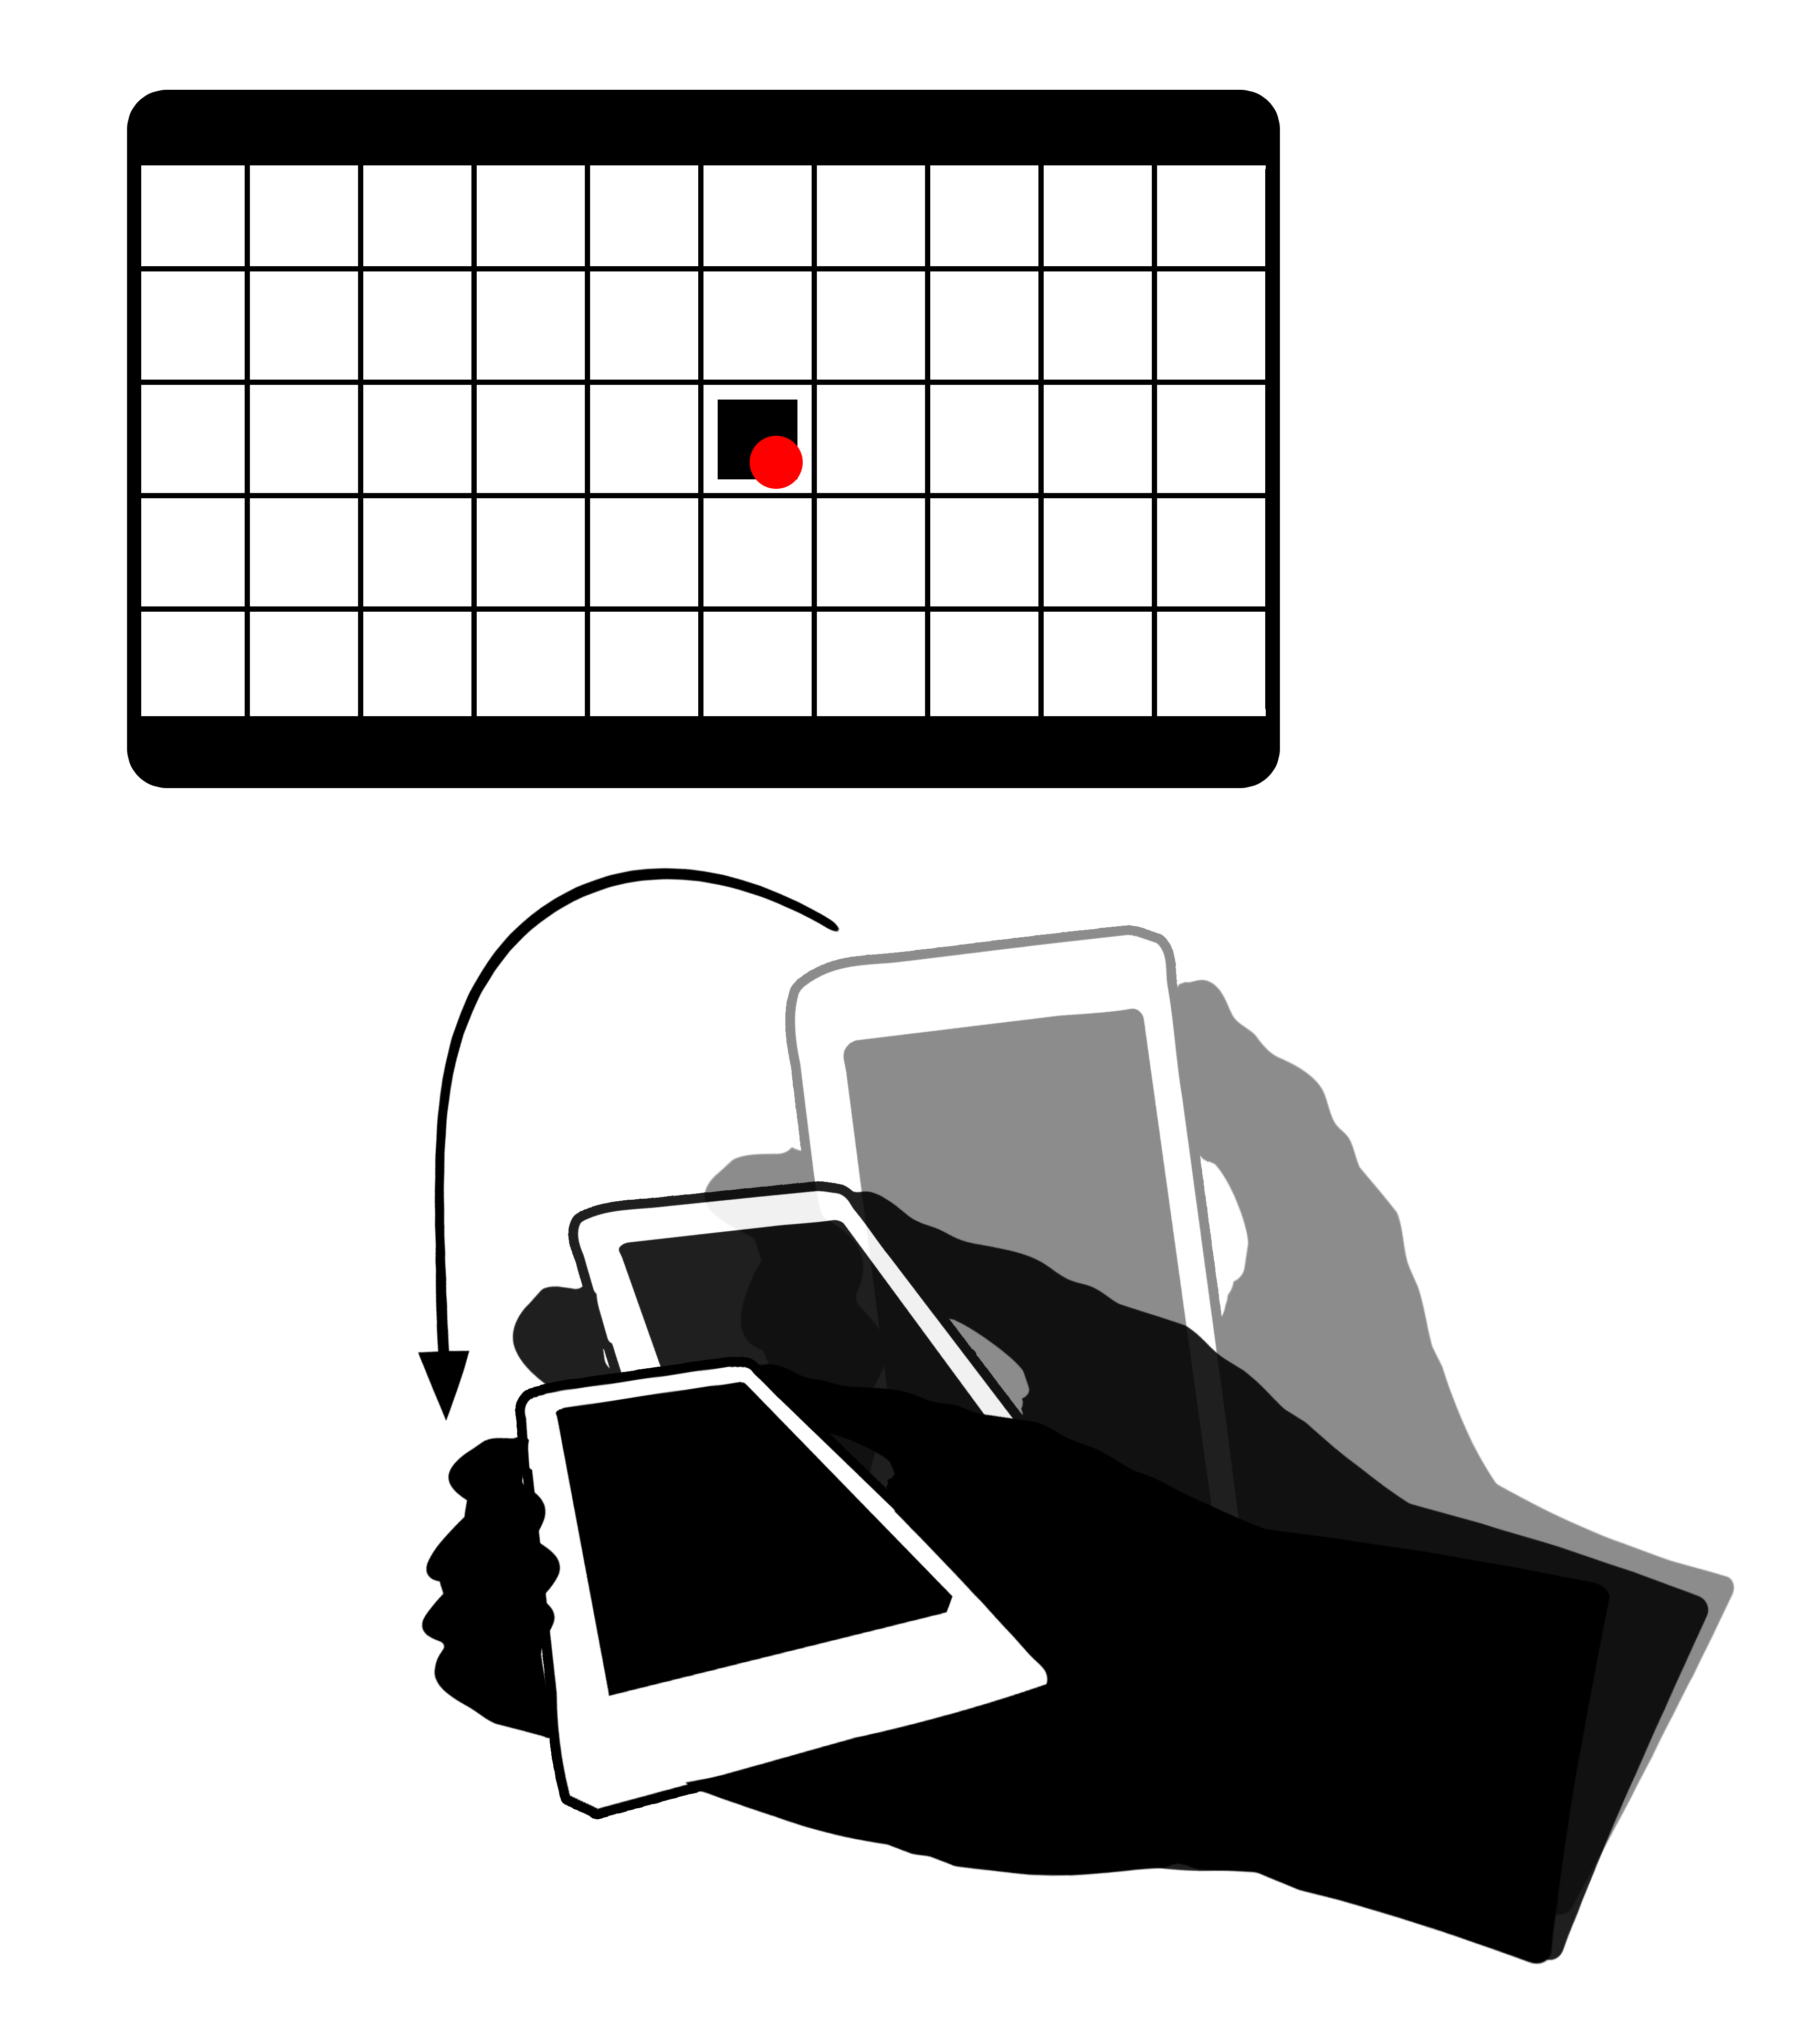
\includegraphics[width = 1\columnwidth]{images/Tilt.jpg}\label{fig:tiltTechnique1}}
\caption{
	\protect\subref{fig:tiltTechnique1} The \tilt technique is performed by doing a forward tilt motion with the phone.
}
\label{fig:tiltTechnique}
\end{figure}

The \throw technique (\Cref{fig:throwTechnique}) is a combination of a technique for pointing \cite{Scheible:2008} i.e. using a hand as a cursor in mid-air, and a throw technique described by Walter et al. \cite{Walter:2014} used in a system for sharing information on large public displays.
We chose to include this technique based on its natural and playful design.
The technique mimics the real world scenario of throwing something like a ball somewhere or to someone.
\throw is two handed, more complex than aforementioned techniques, and takes a little longer to execute because of the increased number of steps.
The \throw technique is performed by 
\begin{enumerate*}[label=\itshape\roman*\upshape)]
	\item{pointing at a target on the large display with one hand (\cref{fig:throwTechnique})} 
	\item{holding the phone in the other hand, and}
	\item{making a swinging motion towards the large display (\cref{fig:throwTechnique}).}
\end{enumerate*}

\begin{figure}[H]
\subfloat[]{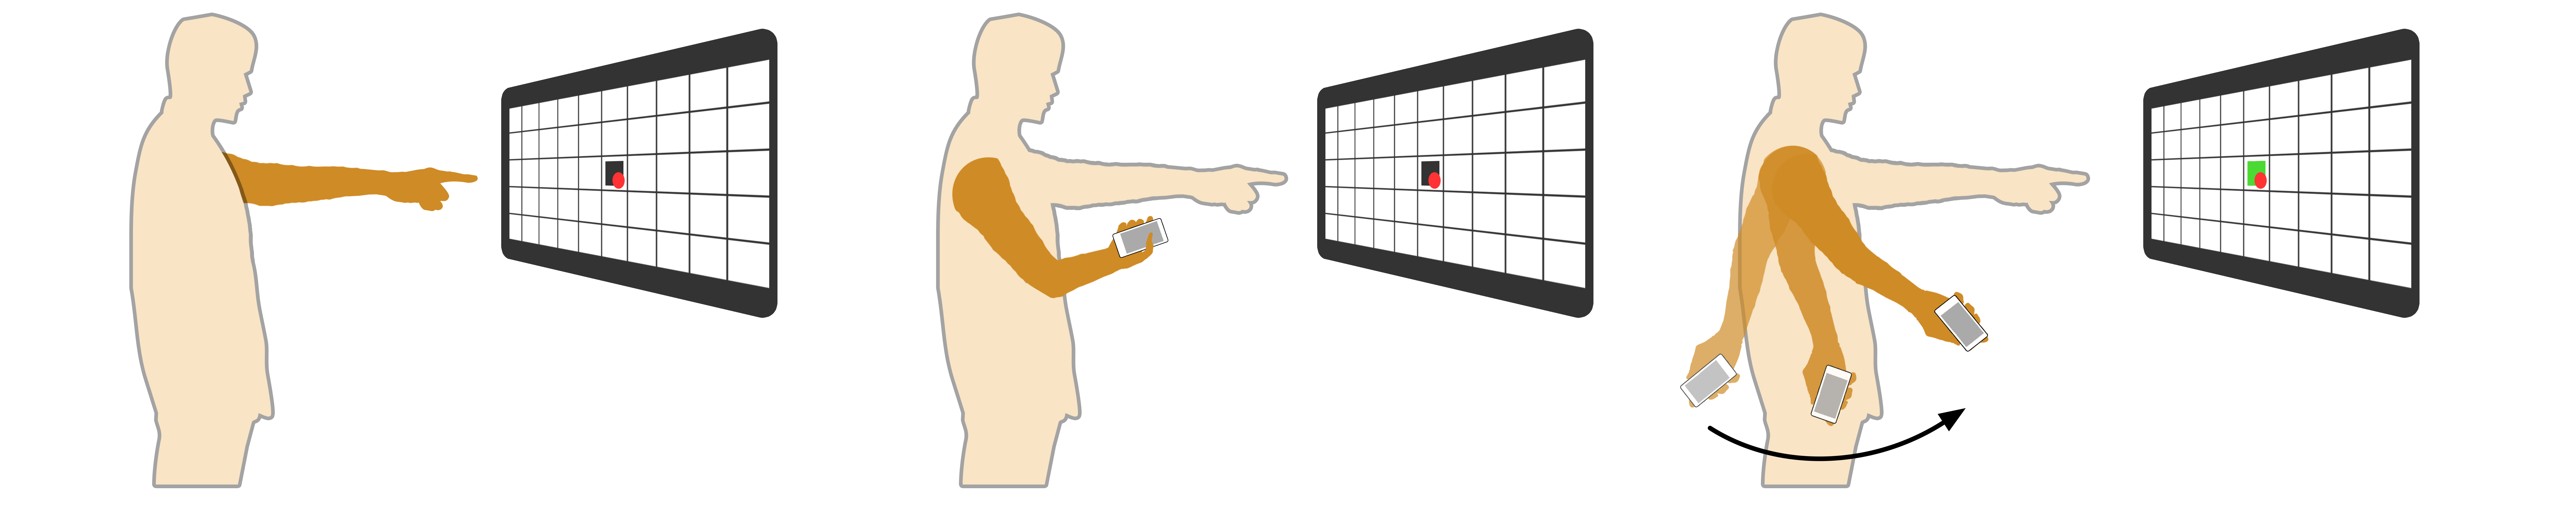
\includegraphics[width = 1\columnwidth]{images/Throw.jpg}\label{fig:throwTechnique1}}
\caption{
	\protect\subref{fig:throwTechnique1} First step of \throw is to point at the screen.
}
\label{fig:throwTechnique}
\end{figure}

The \pinch technique (\Cref{fig:pinchTechnique}) is used in \cite{Ikematsu:2015} by Ikematsu et al., as part of a drag-and-drop method for moving data objects between devices.
Chen et al. uses a pinching gesture in \cite{Chen:2014} for cross-device interaction between a smartphone and a smartwatch to control volume. 
Benko and Wilson \cite{Benko:2010} used the \pinch technique for interacting with an omnidirectional dome.
This technique is again a combination of the pointing technique used by Scheible et al. \cite{Scheible:2008} and the aforementioned pinching techniques. 
The reason for including this technique was to imitate the natural action of picking up a real object e.g. piece of paper, and then moving it to another location.
With \pinch we get a two handed technique which requires the user perform a series of steps and are thus considered more complex and time consuming  than the one handed \swipe and \tilt.
The \pinch technique is performed by 
\begin{enumerate*}[label=\itshape\roman*\upshape)]
	\item{holding the phone in one hand and making a pinch gesture on the phone with the other hand (\Cref{fig:pinchTechnique} 1), subsequently closing the hand}
	\item{pointing at a target on the large display with the closed hand (\cref{fig:pinchTechnique} 2), and}
	\item{opening the hand to complete the technique (\cref{fig:pinchTechnique} 3).}
\end{enumerate*}

\begin{figure}[H]
\subfloat[]{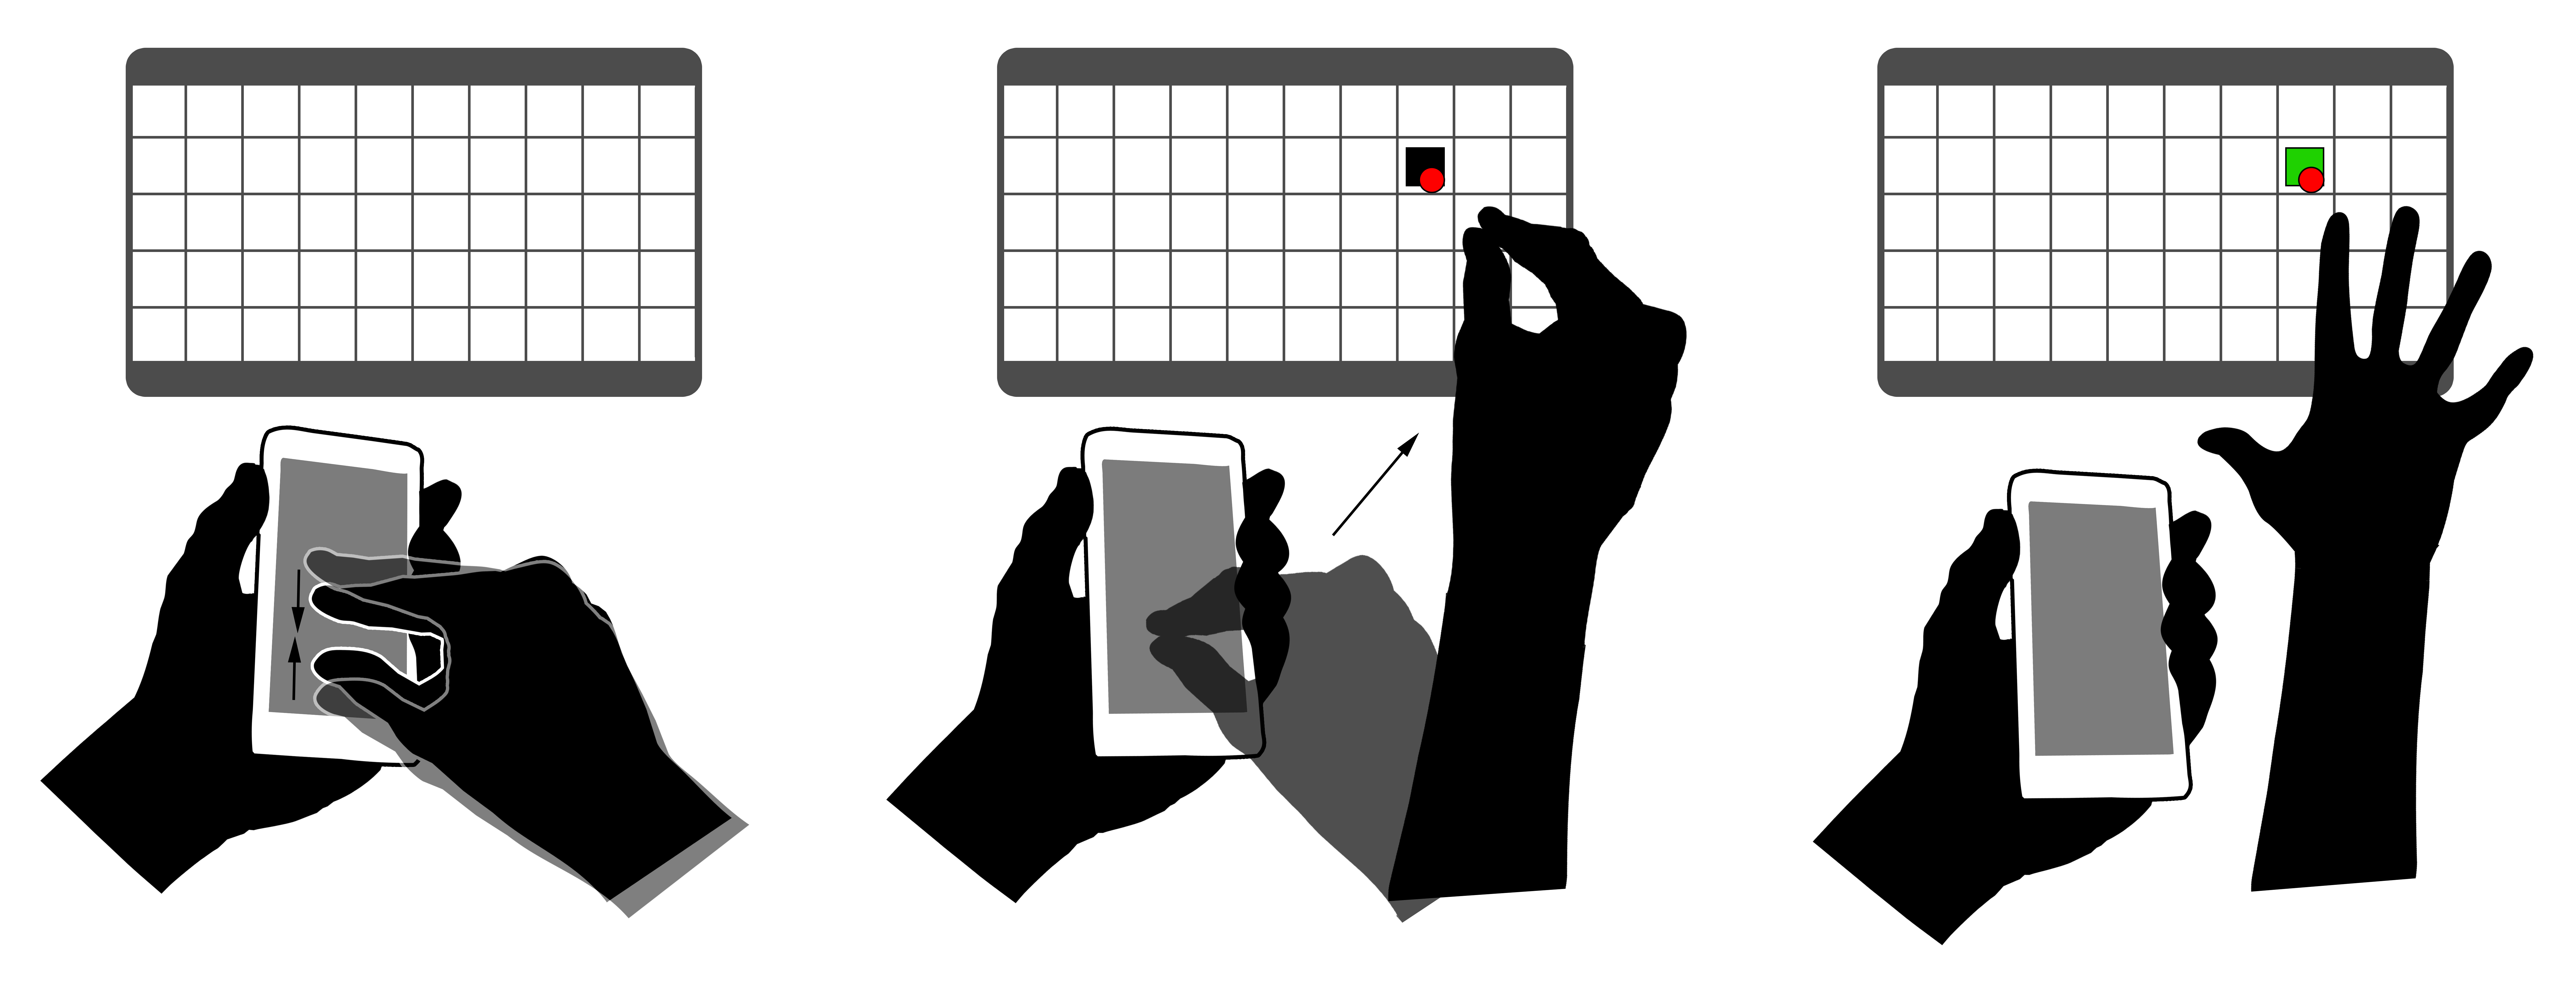
\includegraphics[width = 1\columnwidth]{images/Pinch.jpg}\label{fig:pinchTechnique1}}
\caption{
	\protect\subref{fig:pinchTechnique1} First step of the \pinch technique is to make a pinch gesture on the phone using the index finger and thumb. Second step is to move and use the pinched hand as a pointer.
}
\label{fig:pinchTechnique}
\end{figure}

As mentioned, the techniques have been used in previously published papers where they were part of applications or systems, facilitating interaction between devices such as phone to display interaction and vice versa. 
The described techniques are different in the way they are performed but also the number of hands that are required to make them work.
We chose two techniques that are one-handed (\swipe and \tilt) and two techniques that are two-handed (\throw and \pinch).
Also, to vary the complexity we chose two techniques that require more steps (\throw and \pinch), and two techniques that require less steps for the user to complete the technique (\swipe and \tilt).

All the techniques make use of some combination of pointing in mid-air and touch gestures on the smartphone screen.
The mid-air pointing is achieved by using the Microsoft Kinect for Windows which uses a depth camera making it possible to track a user's hand in mid-air.
As for the touch gestures, smartphones have an accelerometer and a touchscreen, making it possible to detect motion input and detect contact between e.g. a finger and the screen.
These technologies are, in combination with each other, used to recognize the four techniques described in this section. 